\begin{tikzpicture}[remember picture,overlay, shift={(current page.north west)}, >=latex]
	\definecolor{coverblue}{HTML}{8DC73E}%{FF7F49}
	%\definecolor{coverpink}{HTML}{0f97e8}
  \definecolor{coverpink}{HTML}{003d5c}
	\definecolor{coveraccentpink}{HTML}{ffd33c}
	\definecolor{coverorange}{HTML}{ffffff}
	%\definecolor{covershade}{HTML}{0f004d}
  \definecolor{covershade}{HTML}{000000}%{00214a}
\definecolor{c1f958c}{RGB}{31,149,140}
\definecolor{c3ab3cd}{RGB}{58,179,205}
\definecolor{cede632}{RGB}{237,230,50}
\definecolor{c2d70b3}{RGB}{45,112,179}



\begin{slidesonly}
	\begin{scope}
		\node[anchor=south east,inner sep=0pt,outer sep=0pt,] 
		at (current page.south east) {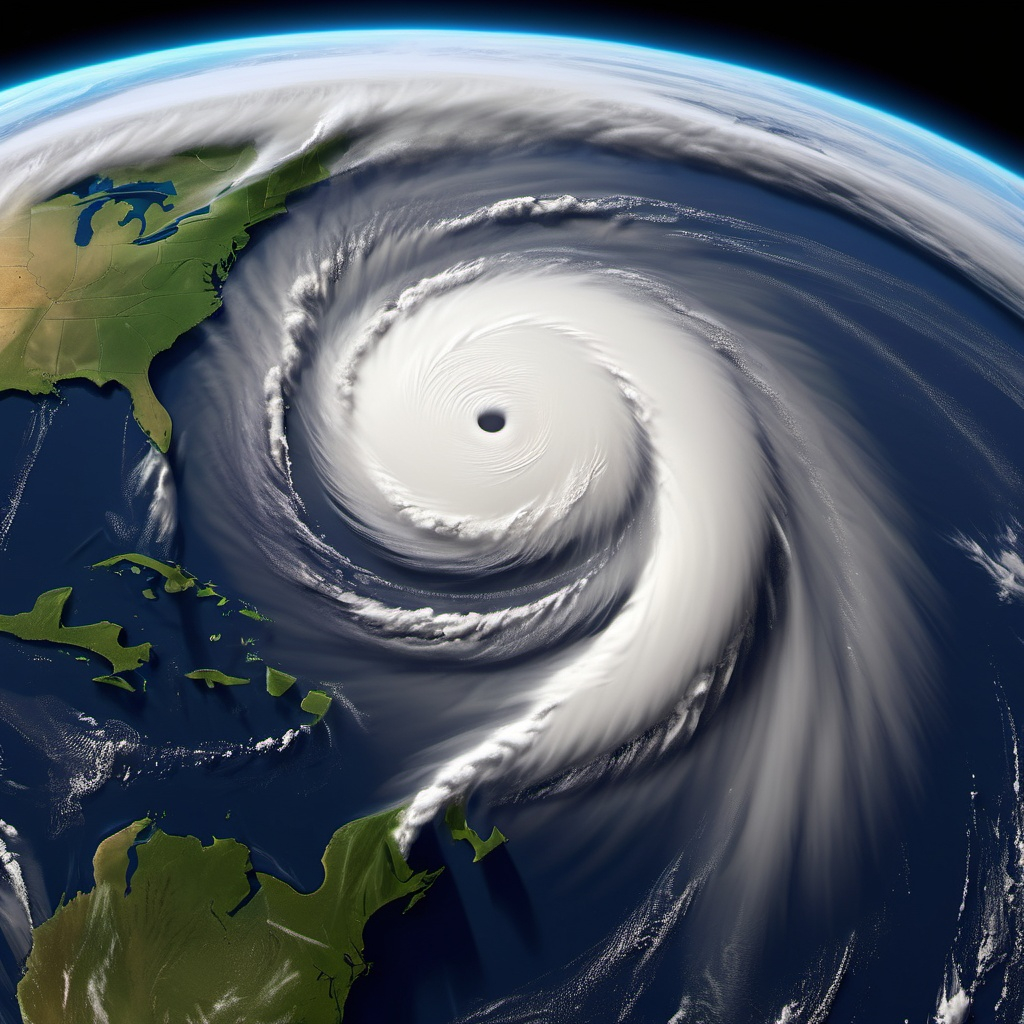
\includegraphics[width=\paperwidth, height=\paperheight]{images/openAIart-hurricane.png}};

%      \begin{scope}[
%        shift={(\pagewidth/2, -15cm)},
%        draw=white,
%        scale=1
%      ]
%        
%        % Define the vector field function
%        % Based on Van der Pol's equation with mu=0.08
%        \def\vectorfieldx(#1,#2){0.08 * (1 - (#2)^2) * (#1) - (#2)}
%        \def\vectorfieldy(#1,#2){(#1)}
%
%        % Draw the vector field
%        \foreach \x in {-10,-9.4,...,10}
%            \foreach \y in {-6,-5.4,...,6}
%            {
%                % Calculate the vector at (\x, \y)
%                \pgfmathsetmacro\vx{\vectorfieldx(\x,\y)}
%                \pgfmathsetmacro\vy{\vectorfieldy(\x,\y)}
%                
%                % Normalize the vector for consistent arrow lengths
%                \pgfmathsetmacro\norm{sqrt(\vx*\vx + \vy*\vy + 0.01)}
%                \pgfmathsetmacro\scaleChange{atan(\norm)/100/\norm}
%                \pgfmathsetmacro\vx{\vx*\scaleChange}
%                \pgfmathsetmacro\vy{\vy*\scaleChange}
%                            
%                % Draw the vector as an arrow
%                \draw[->] (\x,\y) -- ++(\vx,\vy);
%            }
%
%        
%      \end{scope}



		\fill[path fading=north,covershade] (0,2.2in) rectangle ([yshift=-1.01in, xshift=2pt]current page.north east);
		\fill[covershade] (0,-1in) rectangle ([yshift=-1.05in]current page.north east);
%		\fill[path fading=south, covershade] (0,-2in) rectangle ([xshift=1in,yshift=2in]current page.south east);
	\end{scope}
\end{slidesonly}
\begin{bigcover}
	\begin{scope}
		\node[anchor=south east,inner sep=0pt,outer sep=0pt,] 
		at (current page.south east) {\includegraphics[width=\paperwidth, height=\paperheight]{images/Book-cover.pdf}};

%      \begin{scope}[
%        shift={(\pagewidth/2, -15cm)},
%        draw=white,
%        scale=1
%      ]
%        
%        % Define the vector field function
%        % Based on Van der Pol's equation with mu=0.08
%        \def\vectorfieldx(#1,#2){0.08 * (1 - (#2)^2) * (#1) - (#2)}
%        \def\vectorfieldy(#1,#2){(#1)}
%
%        % Draw the vector field
%        \foreach \x in {-10,-9.4,...,10}
%            \foreach \y in {-6,-5.4,...,6}
%            {
%                % Calculate the vector at (\x, \y)
%                \pgfmathsetmacro\vx{\vectorfieldx(\x,\y)}
%                \pgfmathsetmacro\vy{\vectorfieldy(\x,\y)}
%                
%                % Normalize the vector for consistent arrow lengths
%                \pgfmathsetmacro\norm{sqrt(\vx*\vx + \vy*\vy + 0.01)}
%                \pgfmathsetmacro\scaleChange{atan(\norm)/100/\norm}
%                \pgfmathsetmacro\vx{\vx*\scaleChange}
%                \pgfmathsetmacro\vy{\vy*\scaleChange}
%                            
%                % Draw the vector as an arrow
%                \draw[->] (\x,\y) -- ++(\vx,\vy);
%            }
%
%        
%      \end{scope}



		\fill[path fading=north,covershade] (0,2.2in) rectangle ([yshift=-1.01in, xshift=2pt]current page.north east);
		\fill[covershade] (0,-1in) rectangle ([yshift=-1.05in]current page.north east);
%		\fill[path fading=south, covershade] (0,-2in) rectangle ([xshift=1in,yshift=2in]current page.south east);
	\end{scope}		
\end{bigcover}




\newcommand{\titletext}[5]{
	\draw (#1, #2) node[right,opacity=0.55] {	
		\textpdfrender{
		    TextRenderingMode=Fill,
		    LineWidth=1pt,
		    FillColor=#4,
		  }{\fontsize{#5}{100}\fontfamily{phv}\selectfont  \bfseries #3}
	};
	\draw (#1, #2) node[right] {	
		\textpdfrender{
		    TextRenderingMode=Stroke,
		    LineWidth=1pt,
		    StrokeColor=#4,
		  }{\fontsize{#5}{100}\fontfamily{phv}\selectfont  \bfseries #3}
	};
}

\newcommand{\subtitletext}[5]{
	\draw (#1, #2) node[right,opacity=0.55] {	
		\textpdfrender{
		    TextRenderingMode=Fill,
		    LineWidth=1pt,
		    FillColor=#4,
		  }{\fontsize{#5}{100}\fontfamily{phv}\selectfont #3}
	};
	\draw (#1, #2) node[right] {	
		\textpdfrender{
		    TextRenderingMode=Stroke,
		    LineWidth=1pt,
		    StrokeColor=#4,
		  }{\fontsize{#5}{100}\fontfamily{phv}\selectfont #3}
	};
}




  \begin{scope}[yscale=-1, xscale=1, x=2.7pt, y=2.7pt,line join=miter,line cap=butt,line width=1.3pt, yshift=2.3cm, xshift=.7cm,
	  ]

	\coordinate (SUB) at (135, 4);

\begin{bookonly}
	\titletext{6}{-5}{Mathematical Modelling}{coverblue}{50}%{58}	
\end{bookonly}

\begin{displayonly}
	\titletext{6}{-5}{Mathematical Modelling}{coverblue}{45}%{50}	
\end{displayonly}


%    \begin{scope}[yscale=-9.7, xscale=9.7, yshift=-.96in]
%	  \fill[coverblue, opacity=.7] \LINEARALGEBRAoutline;
%	  \draw[coverblue, line width=1.3pt] \LINEARALGEBRAoutline;
%    \end{scope}
  \end{scope}
%


  

	\path[white] (SUB) node[anchor=north west] {\Large \bfseries \sffamily \coversubtitle};



\newcommand{\authornames}{\huge \sffamily \bfseries \begin{tabular}{r}Bernardo Galv\~ao-Sousa\end{tabular}}
	\newcommand{\ypadd}{.5em}
	\newcommand{\xpadd}{1em}


\begin{bookonly}
	\draw (0, 15) node[right, xshift=10em] (AUTHOR) {\phantom{\authornames}};	
\end{bookonly}
\begin{bigcover}
	\draw (0, -25) node[right, xshift=10em] (AUTHOR) {\phantom{\authornames}};		
\end{bigcover}

\begin{displayonly}
	\draw (0, -8.5) node[right, xshift=10em] (AUTHOR) {\phantom{\authornames}};	
\end{displayonly}

\begin{slidesonly}

	\path let \p1 = (AUTHOR.north) in coordinate (Ab1) at (0,\y1+\ypadd);
	\path let \p1 = (AUTHOR.north east) in coordinate (Ab2) at (\x1+\xpadd,\y1+\ypadd);
	\path let \p1 = (AUTHOR.south east) in coordinate (Ab3) at (\x1+\xpadd,\y1-\ypadd);
	\path let \p1 = (AUTHOR.south) in coordinate (Ab4) at (0,\y1-\ypadd);

	\path[fill=covershade, path fading=west, opacity=.8] (Ab1) -- (Ab2) -- (Ab3) -- (Ab4);
	\draw[covershade!80!black, line width=1.3pt] (Ab1) -- (Ab2) -- (Ab3) -- (Ab4);
	
	\draw (0, -8.5) node[right, xshift=10em, white!75!black] (AUTHOR) {\authornames};	
\end{slidesonly}

\begin{bookonly}
	\draw (0, 15) node[right, xshift=10em, white!75!black] (AUTHOR) {\authornames};
\end{bookonly}
\begin{bigcover}
	\path let \p1 = (AUTHOR.north) in coordinate (Ab1) at (0,\y1+\ypadd-470);
	\path let \p1 = (AUTHOR.north east) in coordinate (Ab2) at (\x1+\xpadd,\y1+\ypadd-470);
	\path let \p1 = (AUTHOR.south east) in coordinate (Ab3) at (\x1+\xpadd,\y1-\ypadd-470);
	\path let \p1 = (AUTHOR.south) in coordinate (Ab4) at (0,\y1-\ypadd-470);

	\path[fill=covershade, path fading=west, opacity=.8] (Ab1) -- (Ab2) -- (Ab3) -- (Ab4);
	\draw[covershade!80!black, line width=1.3pt] (Ab1) -- (Ab2) -- (Ab3) -- (Ab4);

	\draw (0, -25) node[right, xshift=10em, white!75!black] (AUTHOR) {\authornames};
\end{bigcover}

\end{tikzpicture}
